\documentclass[12pt]{article}
\usepackage[left=0.25cm,top=1cm,right=0.25cm,bottom=1cm]{geometry}
\textwidth = 20cm
\hoffset = -1cm
\usepackage[utf8]{inputenc}
\usepackage[spanish,es-tabla]{babel}
\usepackage[autostyle,spanish=mexican]{csquotes}
\usepackage[tbtags]{amsmath}
\usepackage{nccmath}
\usepackage{amsthm}
\usepackage{amssymb}
\usepackage{graphicx}
\usepackage{standalone}
\usepackage[outdir=./]{epstopdf}
\usepackage{siunitx}
\usepackage{physics}
\usepackage{color}
\usepackage{float}
\usepackage{multicol}
%\usepackage{milista}
\usepackage{enumitem}
\usepackage{anyfontsize}
\usepackage{anysize}
\usepackage{enumitem}
\usepackage{capt-of}
\usepackage{bm}
\usepackage{relsize}
\usepackage{placeins}
\usepackage{empheq}
\usepackage{cancel}
\usepackage{wrapfig}
\spanishdecimal{.}
\renewcommand{\baselinestretch}{1.5} 
\renewcommand\labelenumii{\theenumi.{\arabic{enumii}}}
\newcommand{\ptilde}[1]{\ensuremath{{#1}^{\prime}}}
\newcommand{\stilde}[1]{\ensuremath{{#1}^{\prime \prime}}}
\newcommand{\ttilde}[1]{\ensuremath{{#1}^{\prime \prime \prime}}}
\newcommand{\ntilde}[2]{\ensuremath{{#1}^{(#2)}}}


\title{Clasificación de las EDP} \vspace{-3ex}
\author{M. en C. Gustavo Contreras Mayén}
\date{ }
\newcommand{\Cancel}[2][black]{{\color{#1}\cancel{\color{black}#2}}}
\begin{document}
\vspace{-4cm}
\maketitle
\fontsize{14}{14}\selectfont
\tableofcontents
\newpage

\section{Ecuaciones Diferenciales Parciales}
\subsection{Introducción}

La mayoría de los fenómenos físicos, ya sea en el dominio de la dinámica de fluidos, la electricidad, el magnetismo, la mecánica clásica o cuántica, la óptica o el flujo de calor, pueden describirse en general mediante \emph{ecuaciones diferenciales parciales} (EDP).
\par
Encontraremos que la mayoría de la física matemática son EDP. Es cierto que se pueden hacer simplificaciones que reduzcan las ecuaciones en cuestión a ecuaciones diferenciales ordinarias, sin embargo, la descripción completa de estos sistemas reside en el área general de la matemática para las EDP.

\subsection{Definición}

Una ecuación diferencial parcial (EDP) es una ecuación que contiene derivadas parciales. 
\par
En contraste con las ecuaciones diferenciales ordinarias (EDO), donde la función desconocida depende solo de una variable, en las EDP, la función desconocida depende de varias variables (como la temperatura $u (x, t)$ depende tanto de la posición $x$ como del tiempo $t$).
\par
Para simplificar la escritura, haremos uso indistintamente de la siguiente notación:
\begin{align*}
u_{t} = \pdv{u}{t} \hspace{1cm} u_{x} = \pdv{u}{x} \hspace{1cm} u_{xx} = \pdv[2]{u}{x} \hspace{1cm} u_{xy} = \pdv[2]{u}{x}{y}
\end{align*}

Enumeremos algunas EDP conocidas:
\begin{align*}
u_{t} &= u_{xx} \hspace{2.25cm} \mbox{Ec. de calor en 1D} \\[0.5em] 
u_{t} &= u_{xx} + u_{yy} \hspace{1cm} \mbox{Ec. de calor en 2D} \\[0.5em] 
u_{rr} &+ \dfrac{1}{r} \, u_{r} + \dfrac{1}{r^{2}} \, u_{\theta \theta} = 0 \\[0.5em]
&{} \mbox{Ec. de Laplace en coord. polares} \\[0.5em]
u_{tt} &= u_{xx} + u_{yy} + u_{zz} \hspace{1cm} \mbox{Ec. de onda en 3D} \\[0.5em] 
u_{tt} &= u_{xx} + \alpha \, u_{t} + \beta \, u \hspace{0.9cm} \mbox{Ec. del telégrafo}
\end{align*}

Veamos de los ejemplos anteriores que la función desconocida $u$ siempre depende de más de una variable.
\par
La variable $u$ (que diferenciamos) se llama \textbf{variable dependiente}, mientras que aquellas con respecto a las que diferenciamos se llaman \textbf{variables independientes}.
\par
Por ejemplo, de la ecuación:
\begin{align*}
u_{t} = u_{xx}
\end{align*}

la variable dependiente $u(x, t)$ es una función de dos variables independientes $x$ y $t$.

Mientras que para la ecuación
\begin{align*}
u_{t} = u_{rr} + \dfrac{1}{r} \, u_{r} + \dfrac{1}{r^{2}} \, u_{\theta \theta}
\end{align*}

se tiene que $u(r, \theta, t)$ depende de las variables $r$, $\theta$ y $t$.

\subsection{¿Por qué son importantes las EDP?}

La mayoría de las leyes naturales de la física, como las ecuaciones de Maxwell, la ley de enfriamiento de Newton, las ecuaciones de Navier-Stokes, las ecuaciones de movimiento de Newton y la ecuación de Schrödinger de la mecánica cuántica, se expresan (o pueden ser expresadas) en términos de EDP, es decir, estas leyes describen los fenómenos físicos relacionando las derivadas espaciales y temporales.
\par
Las derivadas se presentan en estas ecuaciones porque las derivadas modelan cosas naturales (como velocidad, aceleración, fuerza, fricción, flujo, corriente). 
\par
Por tanto, tenemos ecuaciones que relacionan derivadas parciales de alguna cantidad desconocida que nos gustaría encontrar.

\section{Tipos de EDP}
\subsection{Clasificación}

Las ecuaciones diferenciales parciales se clasifican de acuerdo a ciertas características que presentan. La clasificación es un concepto importante porque la teoría general y \emph{los métodos de solución generalmente se aplican solo a una clase determinada} de ecuaciones.

\subsection*{Orden de la EDP}

El orden de una EDP es el orden de la derivada parcial más alta, por ejemplo
\begin{align*}
u_{t} &= u_{xx} \hspace{3.3cm} \mbox{es de segundo orden} \\[0.5em] 
u_{t} &= u_{x} \hspace{3.5cm} \mbox{es de primer orden} \\[0.5em] 
u_{t} &= u \, u_{xx} + \sin x \hspace{1.4cm} \mbox{es de tercer orden}
\end{align*}

\subsection*{No. de variables}

El número de variables es el número de variables independientes, por ejemplo
\begin{align*}
u_{t} &= u_{xx} \hspace{3cm} \hspace{1.61cm} \mbox{dos variables: } x, t \\[0.5em] 
u_{t} &= u_{rr} + \dfrac{1}{r} \, u_{r} + \dfrac{1}{r^{2}} \, u_{\theta \theta} \hspace{1.5cm} \mbox{tres variables: } r, \theta, t
\end{align*}

\subsection*{Linealidad}

Las EDP son lineales o no lineales. En las lineales, la variable dependiente $u$ y todas sus derivadas aparecen de forma lineal (no se multiplican juntas ni al cuadrado, por ejemplo).
\par
Más precisamente, una \emph{ecuación lineal de segundo orden en dos variables} es una ecuación de la forma
\begin{align}
\addtolength{\fboxsep}{5pt}\boxed{ A \, u_{xx} + B \, u_{xy} + C \, u_{yy} + D \, u_{x} + E \, u_{y} + F \, u = G}
\label{eq:ecuacion_01_01}
\end{align}

donde $A, B, C, D, E, F$ y $G$ pueden ser \emph{constantes} o \emph{funciones de} $(x, y)$.

Por ejemplo
\begin{align*}
e^{-t} \, u_{xx} + \sin t &= u_{tt} \hspace{2cm} \mbox{(lineal)} \\[0.5em] 
u \, u_{xx} + u_{t} &= 0 \hspace{2cm} \mbox{(no lineal)} \\[0.5em] 
u_{xx} + y \, u_{yy} &= 0 \hspace{2cm} \mbox{(lineal)} \\[0.5em] 
x \, u_{x} + y \, u_{y} + u^{2} &= 0 \hspace{2cm} \mbox{(no lineal)}
\end{align*}

\subsection*{Homegeneidad}

La ec. (\ref{eq:ecuacion_01_01}) se denomina \emph{homogénea} si el lado derecho de la igualdad $G(x, y)$ es cero para todo $x$, e $y$.
\par
Mientras que si $G(x, y)$ no se anula, entonces la ecuación se denomina \emph{no homogénea}.

\subsection*{Tipo de coeficientes}

Si los coeficientes $A, B, C, D, E, F$ en la ec. (\ref{eq:ecuacion_01_01}) son constantes, entonces (\ref{eq:ecuacion_01_01}) tiene \emph{coeficientes constantes}, de otra manera, la ecuación tiene \emph{coeficientes variables}.

\subsection{Tres tipos de EDP}

Toda EDP lineal como la ec. (\ref{eq:ecuacion_01_01}) puede clasificarse como de tipo:
\begin{enumerate}
\item Parabólico.
\item Hiperbólico.
\item Elíptico.
\end{enumerate}

Las ecuaciones \textbf{parabólicas} describen por ejemplo el flujo de calor y procesos de difusión, además satisfacen la propiedad $B^{2} - 4 \, A \, C = 0$.
\par
Las ecuaciones \textbf{hiperbólicas} describen sistemas que vibran así como el movimiento de las ondas, satisfacen la propiedad $B^{2} - 4 \, A \, C > 0$.
\par
Las ecuaciones \textbf{elípticas} describe fenómenos estacionarios y satisfacen la propiedad $B^{2} - 4 \, A \, C < 0$.

Como ejemplo veamos:
\begin{enumerate}
\setlength\itemsep{1em}
\item $u_{t} = u_{xx}$ \hspace{1cm} $B^{2} - 4 \, A \, C = 0$ \hspace{1cm} (parabólica)
\item $u_{tt} = u_{xx}$ \hspace{0.8cm} $B^{2} - 4 \, A \, C = 4$ \hspace{1cm} (hiperbólica)
\item $u_{\xi \eta} = 0$ \hspace{1cm} $B^{2} - 4 \, A \, C = 1$ \hspace{1cm} (hiperbólica)
\item $u_{xx} + u_{yy} = 0$ \hspace{1cm} $B^{2} - 4 \, A \, C = -4$ \hspace{0.6cm} (elíptica)
\item $y \, u_{xx} + u_{yy} = 0$ \hspace{0.6cm} $B^{2} - 4 \, A \, C = - 4 \, y$ 
\\
donde $\begin{cases}
\mbox{elíptica para } y > 0 \\
\mbox{parabólica para } y = 0 \\
\mbox{hipérbolica para } y < 0 \\
\end{cases}$
\newline
En el caso de coeficientes variables, el tipo de ecuación cambia de punto a punto.
\end{enumerate}

\subsection*{Consideraciones}

En general, $B^{2} - 4 \, A \, C$ es una función de las variables independientes; por lo tanto, una ecuación puede cambiar de un tipo básico a otro en todo el dominio de la ecuación (aunque no es común).
\par
La ecuación lineal general (\ref{eq:ecuacion_01_01}) se escribió con variables independientes $x$ e $y$. En muchos problemas, una de las dos variables representa el tiempo, por lo tanto, se escribiría en términos de $x$ y $t$.
\par
En la figura (\ref{fig:figura_clasificacion_EDP}) se muestra un diagrama de clasificación general para las EDP, nuevamente aclaramos que no es una clasificación definitiva, pero engloba algunas características generales que hemos revisado.
\begin{figure}[H]
    \centering
    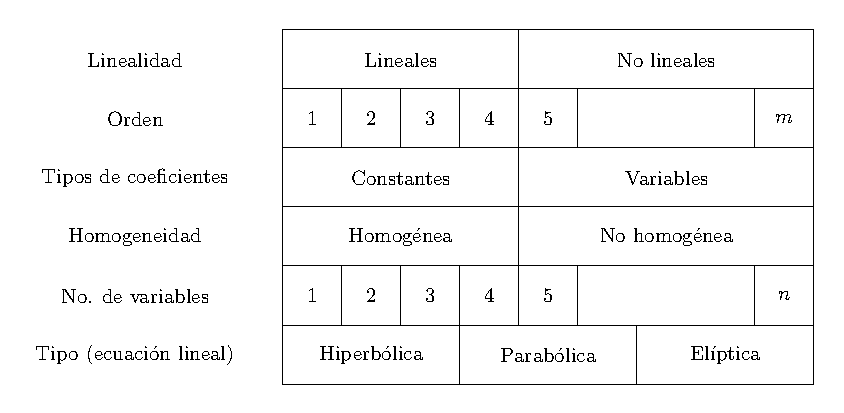
\includegraphics[scale=0.87]{Imagenes/Cuadro_Clasificacion_EDP.eps}
    \caption{Diagrama de clasificación de EDP.}
    \label{fig:figura_clasificacion_EDP}
\end{figure}
\end{document}